\section{Типы индексов}

\subsection{B-tree-индексы}

Когда говорят об индексе без упоминания типа, обычно имеют в виду B-Tree индексы, в которых для хранения данных используется структура, называемая B-tree. Во многих подсистемах хранения на самом деле используются индексы типа B+Tree, в которых каждый листовой узел содержит указатель на следующий для ускорения обхода дерева по диапазону значений.

Общая идея B-дерева заключается в том, что значения хранятся по порядку, и все листовые страницы находятся на одинаковом расстоянии от корня. На рисунке \ref{img:btree-structure} показано абстрактное представление B-Tree индекса. B-Tree-индекс ускоряет доступ к данным, поскольку подсистеме хранения не нужно сканировать всю таблицу для поиска нужной информации. Вместо этого она начинает с корневого узла (не показанного на этом рисунке). В корневом узле имеется массив указателей на дочерние узлы, и подсистема хранения переходит по этим указателям. Чтобы найти подходящий указатель, она просматривает значения в узловых страницах, которые определяют верхнюю и нижнюю границы значений в дочерних узлах. В конечном итоге подсистема хранения либо определяет, что искомое значение не существует, либо благополучно достигает листовой страницы.

Поскольку в B-Tree индексах индексированные столбцы хранятся в упорядоченном виде, то они полезны для поиска по диапазону данных. Например, при спуске вниз по дереву индекса, построенного по текстовому полю, значения перебираются в алфавитном порядке, поэтому поиск «всех лиц, чьи фамилии начинаются с буквы от В до Д» оказывается эффективным.

\begin{figure}[H]
  \centering
  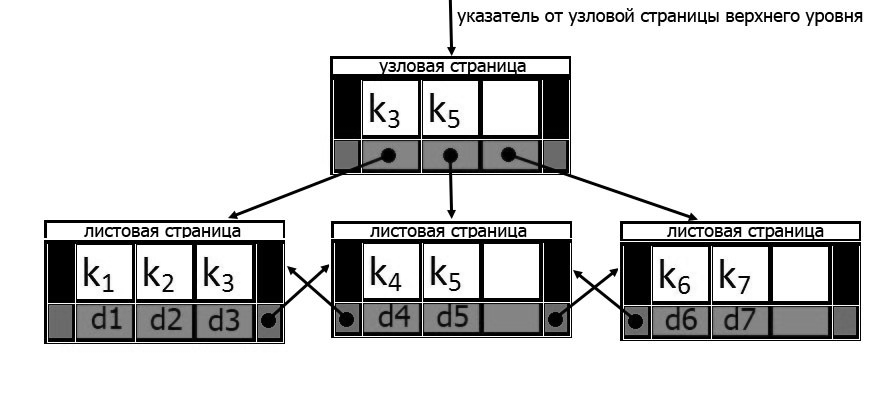
\includegraphics[scale=0.5]{btree.png}
  \caption{Структура данных B+tree.}
  \label{img:btree-structure}
\end{figure}

Где $k_i$ - ключи ($k_i < k_i + 1$), $d_i$ - данные.

Сложность поиска в линейной структуре данных $O(N)$, а в B-tree $O(log(k)+N_k$), где $k$ — количество уровней, а $N_k$ — количество элементов в узле. Поэтому индексы, использующие структуру данных B-tree, эффективны для поиска данных. 

Подсистемы хранения представляют B-Tree-индексы на диске по-разному, и это может влиять на производительность. Например, в MyISAM используется техника сжатия префикса, позволяющая уменьшить размер индекса, а InnoDB не сжимает индексы, поскольку это лишило бы ее возможности выполнять некоторые оптимизации. Кроме того, индексы MyISAM ссылаются на индексированные строки по их физическому адресу на диске, а InnoDB – по значениям первичного ключа. Каждый вариант имеет свои достоинства и недостатки.

\subsection{Хеш-индексы}

Хеш-индекс строится на основе хеш-таблицы и полезен только для точного поиска с указанием всех столбцов индекса. Для каждой строки подсистема хранения вычисляет хеш-код индексированных столбцов – сравнительно короткое значение, которое, скорее всего, будет различно для строк с разными значениями ключей. В индексе хранятся хеш-коды и указатели на соответствующие строки. Т.е. хеш-индексы предполагают хранение не самих значений, а их хэшей, благодаря чему уменьшается размер (а, соответственно, и увеличивается скорость их обработки) индексов из больших полей. Таким образом, при запросах с использованием хеш-индексов, сравниваться будут не искомое со значения поля, а хэш от искомого значения с хэшами полей. 

Из-за нелинейнойсти хэш-функций данный индекс нельзя сортировать по значению, что приводит к невозможности использования в сравнениях больше/меньше и «is null». Кроме того, так как хэши не уникальны, то для совпадающих хэшей применяются методы разрешения коллизий.

Подсистема хранения InnoDB поддерживает так называемые адап­тивные хеш-индексы. Когда InnoDB замечает, что доступ к некоторым значениям индекса происходит очень часто, она строит для них хеш-индекс в памяти, помимо уже имеющихся B-Tree-индексов. Тем самым к B-Tree-индексам добавляются некоторые свойства хеш-индексов, например очень быстрый поиск. Этот процесс полностью автоматический, и вы не можете ни контролировать, ни настраивать его.

\subsection{Полнотекстовые индексы}

В большинстве типичных запросов присутствует фраза WHERE, в которой значения сравниваются на равенство, выделяются диапазоны строк и т. д. Но иногда нужно искать по ключевому слову, и в этом случае поиск должен быть основан на релевантности, а не простом сравнении строк. Для этой цели и предназначены системы полнотекстового поиска. Для полнотекстового поиска требуется специальный синтаксис запроса. Индекс необязателен, но при его наличии поиск выполняется быстрее. Полнотекстовые индексы имеют специальную структуру, ускоряющую поиск документов, содержащих заданные ключевые слова.

Полнотекстовый (FULLTEXT) индекс позволяет искать в тексте ключевые слова, а не сравнивать искомое значение со значениями в столбце. Полнотекстовый поиск не имеет ничего общего с другими типами поиска. С ним связано много тонкостей, например стоп-слова, стемминг, учет множественного числа, а также булевский поиск. Он гораздо больше напоминает поисковые системы, нежели обычное сравнение с критерием во фразе WHERE.

В MySQL поддержка полнотекстового поиска реализована только в подсистеме MyISAM.
